\documentclass{article} 
% \usepackage{iclr2026_conference,times}
\usepackage{macros}
\usepackage{hyperref}
\usepackage{url}
\usepackage[toc,page,header]{appendix}
\usepackage{geometry}
\geometry{margin=1in}

\usepackage{minitoc}

\renewcommand \thepart{}
\renewcommand \partname{}

\title{Spectral State Space Models for Horizontal Connections and Video Modeling}

\author{}

\newcommand{\greg}[1]{{\color{indigo}[Gregoire]: #1}}
\newcommand{\fel}[1]{{\color{gold}[Fel]: #1}}
\newcommand{\agus}[1]{{\color{green}[Agus]: #1}}
\newcommand{\TS}[1]{{\color{pink}[TS]: #1}}
\newcommand{\thomas}[1]{{\color{blue}[Thomas]: #1}}


\begin{document}

\doparttoc % Tell to minitoc to generate a toc for the parts
\faketableofcontents % Run a fake tableofcontents command for the partocs

\maketitle

\begin{abstract}
...
\end{abstract}

\section{Introduction}

\section{Related Work}

\section{Background}

\subsection{Notations}

\greg{TODO : put all vectors and matrices in bold}

\paragraph{Linear Algebra.} Let $\K$ be a field. We identify $\mathcal{M}_{m,n}(\K)$ to $\K^{m \times n}$, the set of $m \!\times\! n$ matrices with coefficients in $\K$. We denote vectors with bold lowercase letters $\bm x \in \K^n$ and linear operators with bold uppercase letters $\bm A \in \K^{m \times n}$. Scalars are denoted with non bold letters. We write $e^A = \sum_{k=0}^\infty \frac{A^k}{k!}$ the matrix exponential, and $\sigma(A)$ the spectrum of $A$.

\paragraph{Special Matrices.} $I_n$ is the identity matrix of size $n$. $\mathrm{Circ}(K) \in \R^{n \times n}$ denotes the circulant matrix generated by the vector $K \in \R^n$, possibly zero padded. $\mathrm{diag}(\Lambda)$ is a diagonal matrix with diagonal $\Lambda \in \R^n$. For ease of notation, we often identify $\Lambda$ and $\mathrm{diag}(\Lambda)$. $\Lambda_c$ is a block-diagonal matrix with blocks of size $c \!\times\! c$. Any matrix $\cdot_c$ notation is block diagonal with blocks of size $c \!\times\! c$. $F_n$ is the Fourier matrix of size $n$.

\paragraph{State Space Models.} For the SSMs, we write $x, y \in \R^{d}$ the input and output, $h \in \R^{N}$ the hidden state, $A \in \R^{{N}\times {N}}$ the transition matrix, $B \in \R^{N \times d}$ and $C \in \R^{d \times N}$ the input and output matrices, respectively. $A$, $\widetilde{A}$ and $\widehat{A}$ denote equivalent formulations of a continuous-time SSM while $\overline{A}$ denotes the discretised version of $A$.

\paragraph{Operators.} As for operators, we use $\otimes$ the Kronecker product, $\circledast$ the block convolution operator, which takes two convolution kernels and produces a new kernel corresponding to the composition of the two convolutions. The size of the resulting kernel is the sum of the sizes of the input kernels minus one. $\ast$ is the convolution operator, which takes a convolution kernel and an input and produces the convolution of the input with the kernel.

\paragraph{Algorithms and Complexity.} $O(\cdot)$ is the big O notation, which hides constant factors and lower order terms. $W$ and $T_\infty$ are the work and time complexity under unlimited parallelism of an algorithm, respectively. Our algorithms require the definition of $(M, \oplus, e)$ a monoid, with $M$ a set, $\oplus$ a binary operation and $e$ the identity element.

\section{Spectral State Space Models}

\paragraph{State Space Model.} The state space model (SSM) is a class of recurrent model with linear recurrent dynamics. Their most general formulation is that of continuous-time (\Cref{eq:ssm}), which can be discretised as in \Cref{eq:ssm:recurrence}, with transition matrices depending on the desired step size following \Cref{eq:zoh}. This continuous time formulation allows the handling of arbitrary sampling rates for free.

\begin{minipage}[t]{.45\linewidth}
  \begin{subequations}
    \label{eq:ssm}
    \begin{align}
      h'(t) &= A h(t) + B x(t) \\
      y(t) &= C h(t) + D x(t)
    \end{align}
  \end{subequations}
\end{minipage}%
\begin{minipage}[t]{.45\linewidth}
  \begin{subequations}
    \label{eq:ssm:recurrence}
    \begin{align}
    \label{eq:ssm:recurrence:1}
      h_{t} &= \overline{A} h_{t-1} + \overline{B} x_t \\
    \label{eq:ssm:recurrence:2}
      y_t &= C h_t + D x_t
    \end{align}
  \end{subequations}
\end{minipage}%

In the remainder of this work, we will omit the residual connection given by $D$ for simplicity.

\paragraph{Discretisation.} Various rules can be used for discretisation, such as the zero-order hold (ZOH) whose solution is given in \Cref{eq:zoh}. $\Delta$ is the time step.
\begin{equation}
\label{eq:zoh}
\overline{A} = e^{\Delta \bm{A}}
\qquad
\overline{B} = (\Delta \bm{A})^{-1} (e^{\Delta \bm{A}} - \bm{I}) \cdot \Delta \bm{B}
\end{equation}

\paragraph{Parallelization.} The crucial property of linear recurrences is that they allow for efficient parallel algorithms. Indeed, sequential computation required by non-linear recurrences is a prohibitive bottleneck for long sequences. In contrast, linear recurrences can be computed using parallel algorithms such as
%
(\emph{i}) the convolutional representation \citep{gu2021efficiently}, which can be computed in $O(T \log T)$ time,
%
(\emph{ii}) the parallel scan (\cref{sec:complexity_analysis}), which also has a logarithmic depth with respect to the sequence length, and
%
(\emph{iii}) the SSD algorithm \citep{TODO}, which relies on structured matrix multiplications.
%
These parallel algorithms allow SSMs to handle long-range dependencies efficiently, making them particularly suitable for tasks such as language modeling and video processing.

\paragraph{Diagonal SSMs.} In the case of scalar inputs and the convolutional representation, \citet{gu2022diagonal} show that if the transition matrix $A$ is well conditioned, computing the convolution kernel only requires knowing its spectrum $\sigma(A)$. More generally, structured matrices allow for efficient computation, with a complexity reduction from $O(N^2)$ to $O(N)$. For any vector-valued input SSM, with $A = P \Lambda P^{-1}$ diagonalizable, we can rewrite the SSM as follows:
%
\begin{align}
\label{eq:ssm:diagonal}
\widetilde{A} = \Lambda \qquad \widetilde{B} = P^{-1} B \qquad \widetilde{C} = C P
\end{align}
These two formulations are equivalent in the sense that they produce the same output $\widetilde{y}(t)=y(t)$, with hidden states linearly related by $\widetilde{h}(t) = P^{-1} h(t)$.

\paragraph{Spectral State Space Models.} We now consider the case where $A$ is block-circulant with blocks of size $c \!\times\! c$. This can be re-writen as a 1D convolution over $\frac{N}{c}$ positions and $c$ channels. Let $F_{\frac{N}{c}} \in \R^{\frac{N}{c} \times \frac{N}{c}}$ be the Fourier matrix. Then, $A$ is diagonalized by $P = F \otimes I_c$, where $\otimes$ is the Kronecker product. It can be written as $A = (F \otimes I_c) \Lambda_c (F^{-1} \otimes I_c)$, where $\Lambda_c$ is a block-diagonal matrix with blocks of size $c \!\times\! c$. The resulting SSM is what we call a Spectral State Space Model (SSSM).

The core idea of SSSMs is to constrain $A$ with a structured change of basis with efficient matrix-matrix and matrix-vector products. This isn't restricted to 1D fourier transforms. For example, this still works when $F_{\frac{N}{c}}$ is replaced by $F_h \otimes F_w$ for 2D convolutions.
%
\begin{align}
\label{eq:ssm:spectral}
\widetilde{A} = \Lambda_c \qquad \widetilde{B} = P^{-1} B \qquad \widetilde{C} = C P
\end{align}

\paragraph{Diagonal SSSMs.} Recall that at this point, we have \Cref{eq:ssm:spectral} where the change of basis is structured. This means that powering $A$ costs $O(\frac{N}{c} c^3) = O(N c^2)$. We go back to the diagonal case where powering $A$ only costs $O(N)$, as this is the bottleneck in parallel algorithms (\cref{app:constant_factors}). We can write $\widetilde{A} = Q_c \Lambda Q_c^{-1}$, where $\Lambda$ is diagonal and $Q_c$ is a block-diagonal matrix with blocks of size $c \!\times\! c$. We get the following diagonal SSM:
%
\begin{align}
\label{eq:ssm:diagonal_spectral}
\widehat{A} = \Lambda \qquad \widehat{B} = Q_c^{-1} P^{-1} B \qquad \widehat{C} = C P Q_c
\end{align}

\section{Convolutional State Space Models}

\paragraph{Motivation.} \greg{Small introductory paragraph about what computational model we ultimately want to reach, and state that we get there through ConvSSMs. Local in space : conv, local in time : SSM. Spatio-temporal model : ConvSSM.}

\subsection{Horizontal Connections}
\label{sec:horizontal_connections}

\paragraph{Computational Motivation.} Many high-dimensional signals, such as images or videos, exhibit strong local spatiotemporal structure. In the context of biological vision, neurons exploit this structure through (\emph{i}) spatial organization, with neurons arranged in a topographic manner that preserves spatial relationships - a property known as retinotopy \citep{TODO} - coupled with (\emph{ii}) local interactions, with neurons primarily connecting to their immediate neighbors in the visual cortex. These local interactions, often referred to as \emph{horizontal connections}, enable information to propagate across space and time while preserving natural structure such as locality.

\paragraph{Algorithmic Motivation.} 
Incorporating spatial dependencies into state space models allows the hidden state to evolve spatio-temporally, enabling the modeling of long-range spatial dependencies through repeated local interactions. This is key for biological plausibility, strong inductive biases, but also for algorithmic efficiency.
%
Indeed, introducing spatial interactions in high-dimensional settings comes with significant computational challenges. For inputs of size $h \!\times\! w \!\times\! c$, the state dimension scales as $N \sim 10^6$. Naively parameterizing dense interaction matrices $A \in \R^{N \times N}$ is therefore intractable, both in terms of work and memory.
%
This necessitates the use of structured operators that reduce complexity while preserving expressivity. In particular, structured matrices admitting fast matrix-vector products are essential to leverage parallel algorithms such as the scan, and to ensure scalability to realistic data regimes.

\paragraph{The ConvSSM.}
Convolutions provide a natural way to reconcile both these computational and algorithmic requirements, which is the reason why they are the de facto standard for modeling spatial interactions in high-dimensional signals - transformers asside. Rewriting the SSM equations (\Cref{eq:ssm}) for kernel convolutions, we get the following spatial convolutional SSM (ConvSSM):

\greg{take ConvS5 notation for the kernels.}

\begin{minipage}[t]{.45\linewidth}
\vspace{-5mm}
  \begin{subequations}
    \label{eq:conv_ssm_continuous}
    \begin{align}
    \label{eq:conv_ssm_continuous:1}
      \frac{\partial h}{\partial t}(r,t) &= K_h \ast h(r, t) + K_x \ast x(r, t) \\
      y(r, t) &= K_y \ast h(r, t)
    \end{align}
  \end{subequations}
\vspace{-5mm}
\end{minipage}%
\begin{minipage}[t]{.45\linewidth}
\vspace{-5mm}
  \begin{subequations}
    \label{eq:conv_ssm_discrete}
    \begin{align}
    \label{eq:conv_ssm_discrete:1}
      h_{t} &= \overline{K}_h \ast h_{t-1} + \overline{K}_x \ast x_t \\
    \label{eq:conv_ssm_discrete:2}
      y_t &= K_y \ast h_t
    \end{align}
  \end{subequations}
\vspace{-5mm}
\end{minipage}

Where $r$ is the spatial position, $K$ are convolution kernels and $\ast$ is the convolution operator. However, the spatial ConvSSM faces two closely linked challenges.
%
(\emph{Challenge A:}) Left in this format, it is not clear how to compute discrete-time kernels $\overline{K}_h$ and $\overline{K}_x$ from their continuous-time counterparts $K_h$ and $K_x$, or what such kernels would even look like. Specifically, \Cref{eq:zoh} requires matrices and cannot be applied to get the discrete-time kernels $\overline{K}_h$ and $\overline{K}_x$.
%
(\emph{Challenge B:}) parallel algorithms break down when adapted to the spatial ConvSSM (\cref{sec:complexity_analysis}).

To circumvent both issues, we move from a spatial to a spectral representation of the ConvSSM. We stack all spatial positions and channels into a single vector, and rewrite the convolutions as matrix-vector products.
%
Indeed, discrete-space convolutions correspond to linear operators with a block-circulant with circulant blocks (BCCB) structure, which are diagonalized by the Fourier transform. This readily fits within the Spectral State Space Model framework introduced in the previous section. We get the following ConvSSM with $d = h w c_\mathrm{in}$-dimensional input and output, and $N = h w c$-dimensional hidden state:
%
\begin{align}
\label{eq:convssm:A}
A &= \mathrm{Circ}(K_h) = P \Lambda^A_c P^{-1} = P Q_c \Lambda Q_c^{-1} P^{-1} \\
\label{eq:convssm:B}
B &= \mathrm{Circ}(K_x) = P \Lambda^B_c P_{\mathrm{in}}^{-1} \\
\label{eq:convssm:C}
C &= \mathrm{Circ}(K_y) = P_{\mathrm{in}} \Lambda^C_c P^{-1}
\end{align}
%
with $P = (F_h \otimes F_w) \otimes I_c$, $P_{\mathrm{in}} = (F_h \otimes F_w) \otimes I_{c_\mathrm{in}}$, $\Lambda$ diagonal and $Q_c$ block-diagonal with blocks of size $c \!\times\! c$. For $B$ and $C$, $\mathrm{Circ}(K)$ is the convolution operator with kernel $K$, and the $\Lambda^{B/C}_c$ are block-diagonal matrices with blocks of size $c \!\times\! c_\mathrm{in}$ and $c_\mathrm{in} \!\times\! c$, respectively, corresponding to the Fourier transform of the convolution kernels.
%
After rewriting the ConvSSM in the spectral domain, all the computational load is absorbed in $B$ and $C$, yielding the following diagonal SSSM:

\begin{align}
\label{eq:convssm}
&\boxed{\widetilde{A} = \Lambda} \\
&\widetilde{B} = Q_c^{-1} P^{-1} P \Lambda^B_c P_{\mathrm{in}}^{-1} = \left(Q_c^{-1} \Lambda^B_c\right) P_{\mathrm{in}}^{-1} \boxed{= \Lambda^{B'}_c P_{\mathrm{in}}^{-1}} \\
&\widetilde{C} = P_{\mathrm{in}} \Lambda^C_c P^{-1} P Q_c = P_{\mathrm{in}} \left(\Lambda^C_c Q_c\right) \boxed{= P_{\mathrm{in}} \Lambda^{C'}_c}
\end{align}

This formulation makes it apparent that the tension in \emph{Challenge A} is that the discretized kernels have full spatial support, rendering the convolutional representation inapplicable. The Spectral ConvSSM trivializes the discretization process through diagonalization, and bypasses prohibitive convolutions through efficient matrix multiplications.
%
Similarly, \emph{Challenge B} also boils down to kernel size explosion, and is bypassed by the spectral formulation for the same reason. We derive the full complexity analysis in \cref{sec:complexity_analysis} and point exactly where the kernel explosion happens for the spatial ConvSSM, and how the spectral formulation avoids~it.

\greg{figure with kernels, block-convolutions of kernels, and $e^{\Delta A}$.}

\paragraph{Link with previous work.}
Previous approaches such as ConvS5 \citep{TODO} faced these challenges by forfeiting horizontal connections. They restrict the transition operator to act independently at each spatial location, typically using $1 \!\times\! 1$ convolutions in \Cref{eq:conv_ssm_continuous}. Equivalently, in the stacked vector representation (\Cref{eq:convssm:A}), this corresponds to replacing the circulant structure of $A$ with a block diagonal with constant blocks $A = I_{hw} \otimes K$ - where $K \in \R^{c \times c}$.

This constraint removes spatio-temporal coupling from the temporal ODE, i.e., the "Conv" in "ConvS5". In contrast, our approach explicitly models spatio-temporal coupling through the spectral domain while retaining the computational benefits of structured state space models.

\subsection{Complexity analysis}
\label{sec:complexity_analysis}

\paragraph{} We focus our analysis on the parallel scan algorithm. We compare in \cref{app:TODO} the parallel scan to the matrix-multiplication based algorithm of SSD \citep{TODO} across a wide range of temporal and spatial regimes.

\paragraph{The Parallel Scan.} In \cref{app:parallel_scan}, we describe the general form of the parallel scan algorithm over a \emph{monoid} $(\mathcal{M}, \oplus, e)$ along with its complexity analysis. We show that \textbf{assuming constant time $\bm \oplus$ operations}, the total \emph{work} of the scan is $O(T)$ with a \emph{time complexity} of $O(\log T)$ under sufficient parallel resources. In the case of SSMs, the monoid is given in \cref{app:SSM_complexity}. Crucially, the corresponding $\oplus$ operation takes constant time, which allows the scan to achieve logarithmic time complexity with respect to the sequence length (\Cref{prop:SSM_complexity}).

\begin{proposition}[SSM Complexity]
\label{prop:SSM_complexity}
    Let $(M, \oplus, e)$ be the monoid corresponding to the SSM, defined by \Cref{eq:M_SSM,eq:+_SSM,eq:0_SSM}. Let $(a_i)_{i\in \intint{0}{T-1}}\in M^{\intint{0}{T-1}}$. Then, the parallel scan over $(a_i)$ has work and time complexity of:
\[
    W(\mathrm{Scan}) = O(T), \qquad T_\infty(\mathrm{Scan}) = O(\log(T))
\]
\end{proposition}

\begin{proof}
See \cref{app:SSM_complexity}.
\end{proof}

\paragraph{Kernel Explosion.} For convolutional SSMs, we can write an equivalent monoid for which the $\oplus$ involves the \emph{block convolution} operator $\circledast$, which takes two convolution kernels and produces a new kernel corresponding to the composition of the two convolutions. The resulting kernel $K_1 \circledast K_2$ has size twice that of its inputs. Concretely, this means that the kernels involved in the scan grow exponentially with the depth of the scan. \Cref{prop:Spatial_ConvSSM_complexity} shows that the final complexity of such a scan is $O(T^2)$ work \textbf{and} time, which is worse than the sequential algorithm.
%
For this reason, \citet{TODO} restrict their ConvS5 model to $1 \!\times\! 1$ convolutions, avoiding algorithmic explosion by cutting all horizontal connections. Even worse, our formulation shows that discretized kernels have full spatial support, meaning that \textbf{even the first step of the scan would be intractable}.

\begin{proposition}[Spatial ConvSSM Complexity]
\label{prop:Spatial_ConvSSM_complexity}
    Let $(M, \oplus, e)$ be the monoid corresponding to the spatial convolutional SSM, defined by \Cref{eq:M_SSM,eq:+_SSM,eq:0_SSM}. Let $(a_i)_{i\in \intint{0}{T-1}}\in M^{\intint{0}{T-1}}$. Then, the parallel scan over $(a_i)$ has work and time complexity of:
\[
    W(\mathrm{Scan}) = T_\infty(\mathrm{Scan}) = O(T^2)
\]
\end{proposition}

\begin{proof}
See \cref{app:Spatial_ConvSSM_complexity}.
\end{proof}

\paragraph{Reaching Criticality.} To monitor this chain reaction of exponentially growing kernels, we can leverage the spectral SSM formulation. Under this framework, the monoid becomes that of \cref{app:Spectral_ConvSSM_complexity}. Crucially, the $\oplus$ operation now only involves diagonal matrix multiplications and produce fixed-size objects. This allows the scan to maintain its logarithmic time complexity, while still modeling horizontal connections (\Cref{prop:Spectral_ConvSSM_complexity}). We discuss in \cref{app:constant_factors} the constant factors hidden in the $O(\cdot)$ notation, and how our framework remains tractable for realistic data regimes.

\begin{proposition}[Spectral ConvSSM Complexity]
\label{prop:Spectral_ConvSSM_complexity}
    Let $(M, \oplus, e)$ be the monoid corresponding to the spectral convolutional SSM, defined by \Cref{eq:M_SSM,eq:+_SSM,eq:0_SSM}. Let $(a_i)_{i\in \intint{0}{T-1}}\in M^{\intint{0}{T-1}}$. Then, the parallel scan over $(a_i)$ has work and time complexity of:
\[
    W(\mathrm{Scan}) = O(T), \qquad T_\infty(\mathrm{Scan}) = O(\log(T))
\]
\end{proposition}

\begin{proof}
See \cref{app:Spectral_ConvSSM_complexity}.
\end{proof}

\subsection{Final Model}
\greg{Find a better section title...}

\paragraph{The Core.} \greg{Spectral ConvSSM}

\paragraph{Parameterization.} \greg{Rework this paragraph} We parameterize $A$ as a complex-valued vector $\Lambda \in \C^N$. As for $B$ and $C$, we can either parameterize them as kernels in the spatial domain, or as block-diagonal matrices in the spectral domain.
%
The spatial parameterization leads to input and output transforms of $O(c c_\mathrm{in} k^2)$ parameters and either $\underbrace{O(hwk^2cc_\mathrm{in})}_{\text{spatial convolution}} + \underbrace{O(hw \log(hw) c)}_{\text{FFT}}$ or $\underbrace{O(hwcc_\mathrm{in})}_{\text{spectral product}} + \underbrace{O(hw \log(hw) c c_\mathrm{in})}_{\text{FFT}}$ complexities depending on the order of operations.
%
The spectral parameterization leads to $O(hwcc_\mathrm{in})$ parameters with complexity of $O(hwcc_\mathrm{in})$.

\paragraph{Stability.} \greg{eigenvalues of $A$}

\paragraph{Circuits.} \greg{All circuit derivation on the SSM applies to our core. We take Gated Delta Net as state of the art circuit and plug it on top of our core.}

\section{Scaling Laws}

\section{Benchmarks}

\section{Fine Tuning for Video Modeling}

\section{Interpretability}

\section{Conclusion}

\bibliography{references}
\bibliographystyle{plainnat}

\newpage
\appendix

\section{Complexity Proofs}
\label{app:complexity_proofs}

We analyse the complexity of the parallel scan algorithm to show why convolutions in spatial domain make the complexity explode, and how doing convolutions in spectral domain preserves $O(\log T)$ complexity. We consider both the work complexity $W$, measuring the total amount of atomic operations to perform, and the time complexity under unlimited parallelization $T_\infty$, measuring the longest sequence of atomic operations remaining after optimal parallelization.

We begin by addressing the main issue of the complexity explosion of convolutional SSMs in \cref{app:parallel_scan,app:SSM_complexity,app:Spatial_ConvSSM_complexity,app:Spectral_ConvSSM_complexity}. Our main result is \Cref{prop:Spectral_ConvSSM_complexity}. We show in \cref{app:Spectral_ConvSSM_complexity} that we can achieve the same work and time complexity as a regular linear SSM. We then tackle the question of reducing the constant to make it tractable, using standard tricks, adapted to our framework, in \cref{app:constant_factors}.

\subsection{The Parallel Scan}
\label{app:parallel_scan}

We first describe the parallel scan operation in the most general way. This operation is the core of the SSM parallelization. Let $(a_i)_{i\in I}\in M^I$ be elements of a monoid $(M,\oplus,e)$, with $I=\intint{0}{T\!-\!1}$. The parallel scan is an algorithm that computes $(s_i=\sum_{j=0}^ia_j)_i\in I$. This algorithm is parallelisable and requires associativity of the $\oplus$ operator and a neutral element $e$, hence the minimal requirement of a monoid structure. It proceeds in two sweeps mirroring each other. The first sweep proceeds in a tree like structure, with level $l$ of the tree computing $a^{l+1}_{k}\coloneqq a^l_{2k} \oplus a^l_{2k+1}$, and initialised with $a^0_k\coloneqq a_k$. Once this upward sweep is over, the downward sweep computes mirror operations, with $b^0_1\coloneqq e$ and $(b^{l+1}_{2k}, b^{l+1}_{2k+1}) = (b^{l}_{k}, b^{l}_{k} \oplus a^{\log_2(T)-(l+1)}_{2k})$. The order is crucial here as $\oplus$ is not required to be commutative. It is only required to be associative. In our application for SSM, it is not be commutative. We denote the parallel scan procedure as $\mathrm{Scan}((a_i)_{i\in I})$ or $\mathrm{Scan}$ for short.
\Cref{fig:parallel_scan_general} provides a visualisation of the entire procedure.

\begin{figure}[ht]
    \centering
    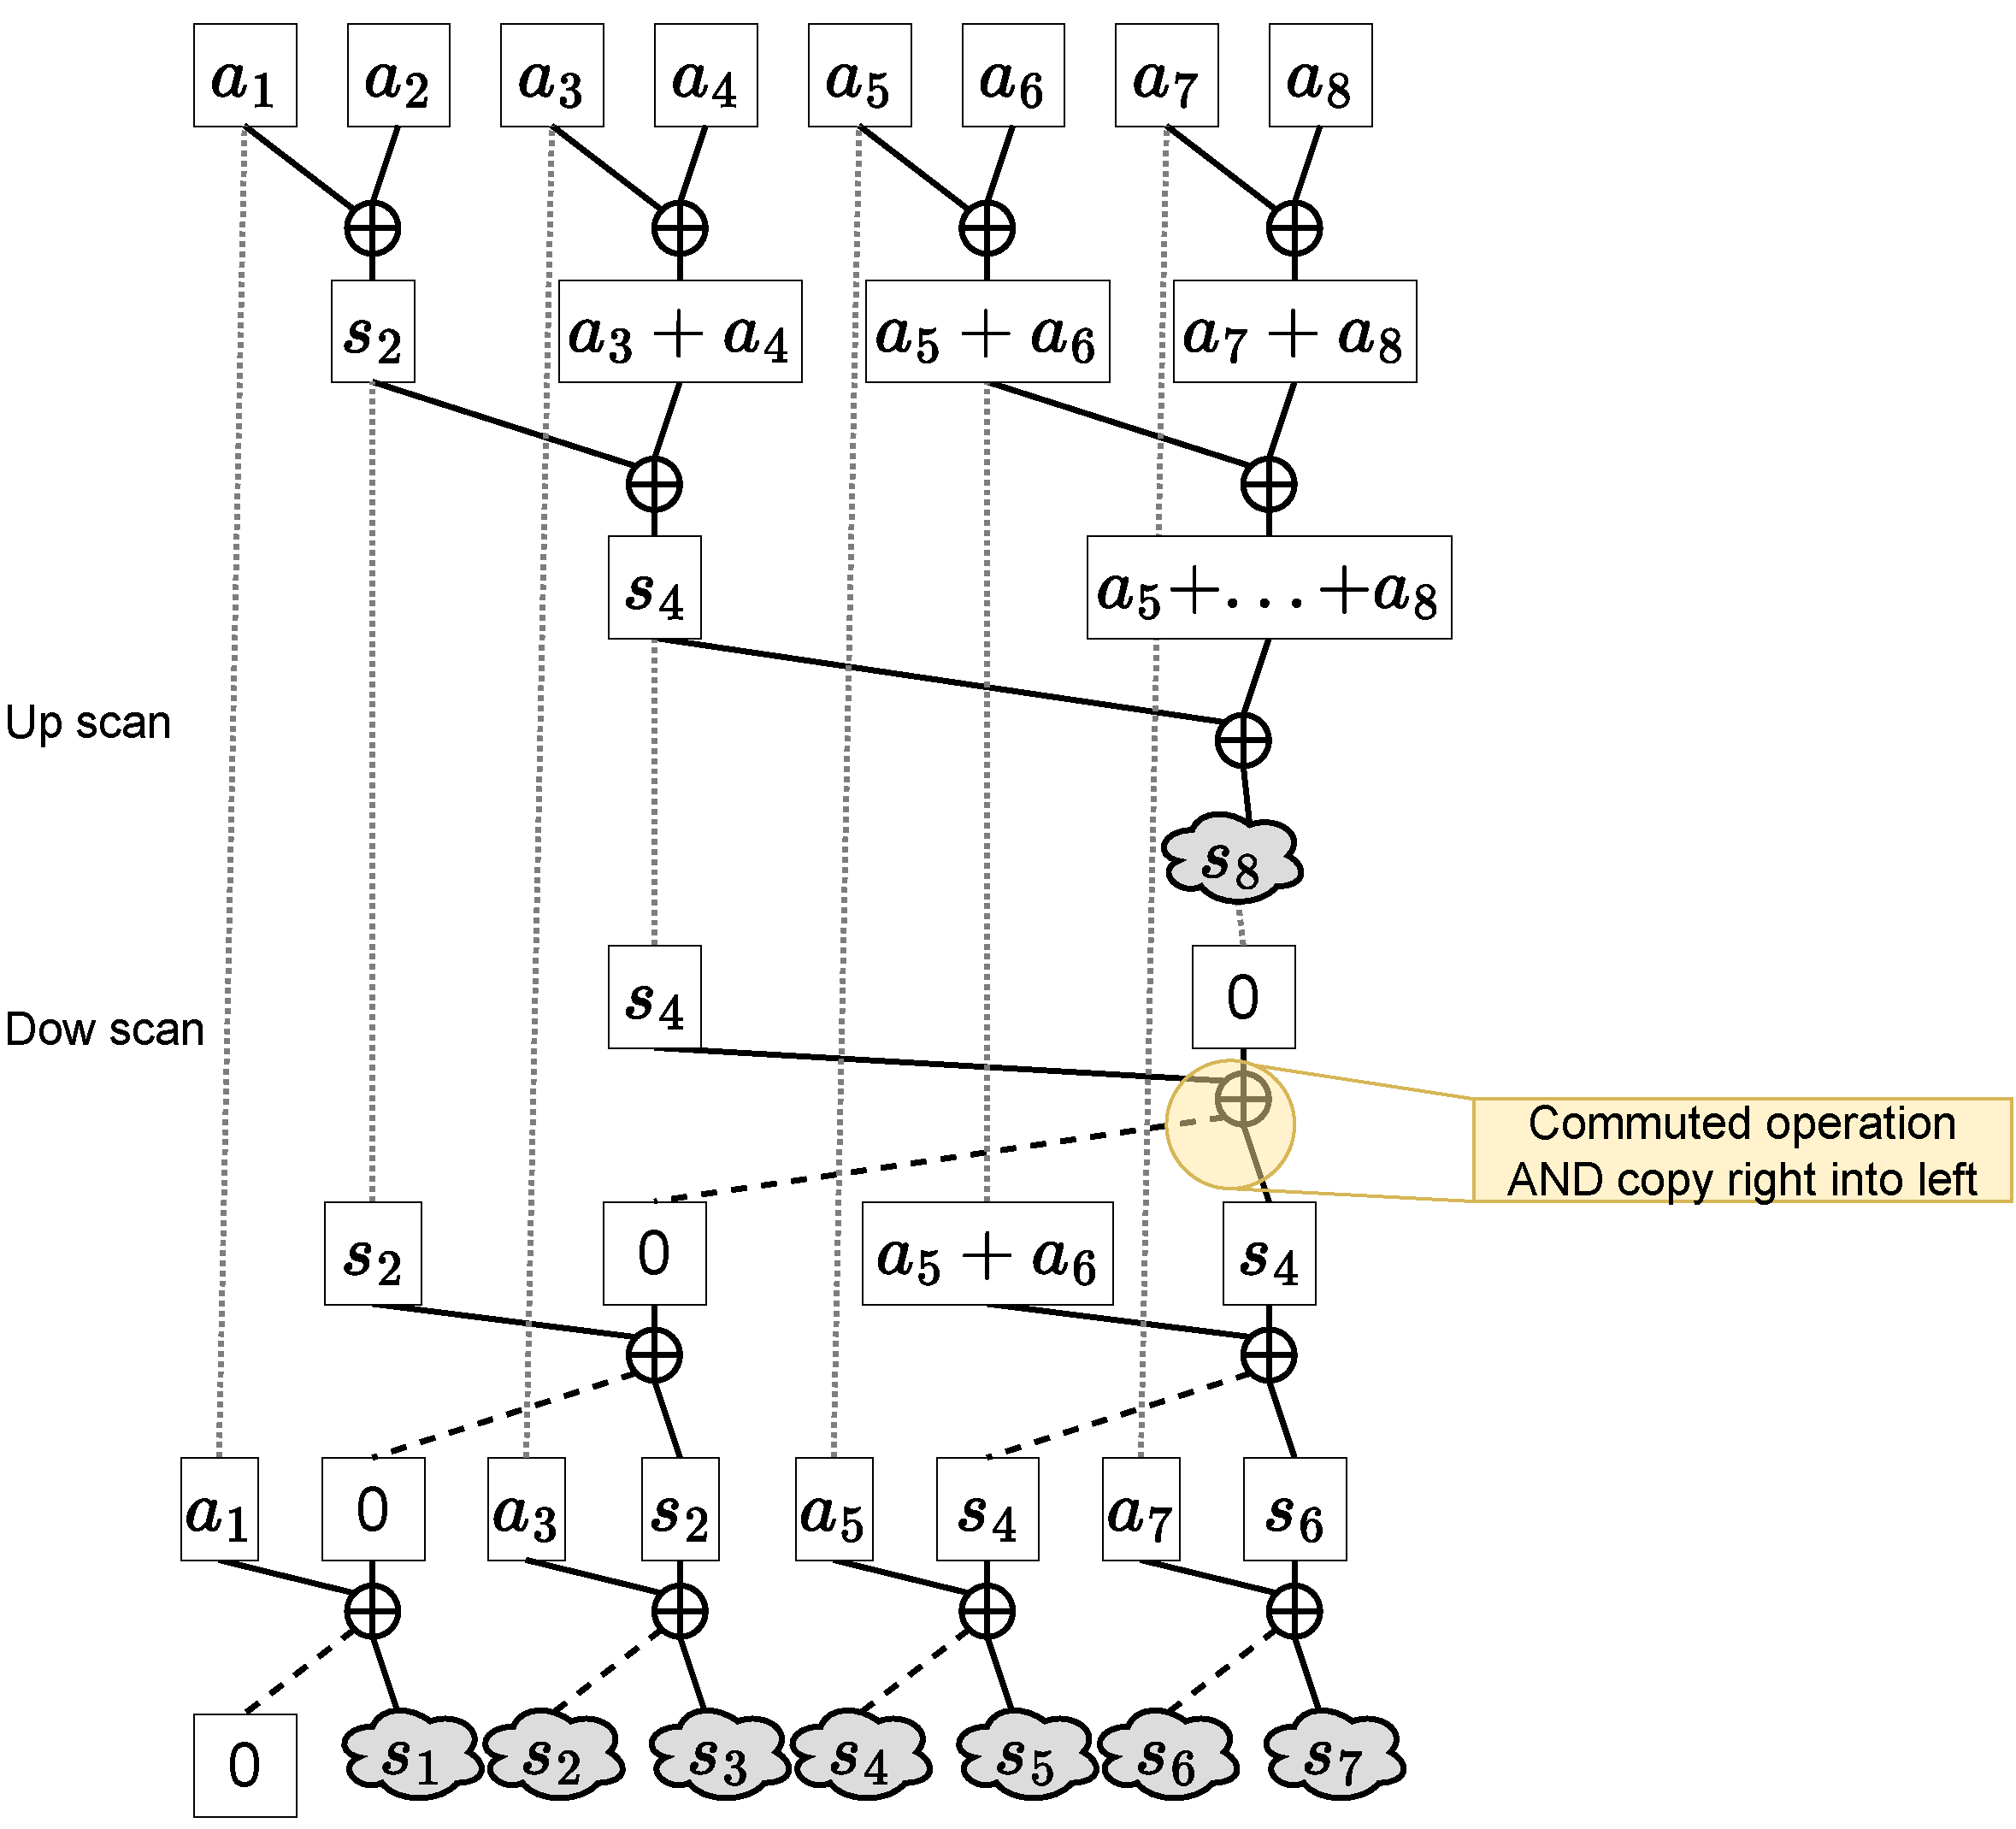
\includegraphics[height=0.3\textheight]{figures/scan_monoid.pdf}
    \hspace{20mm}
    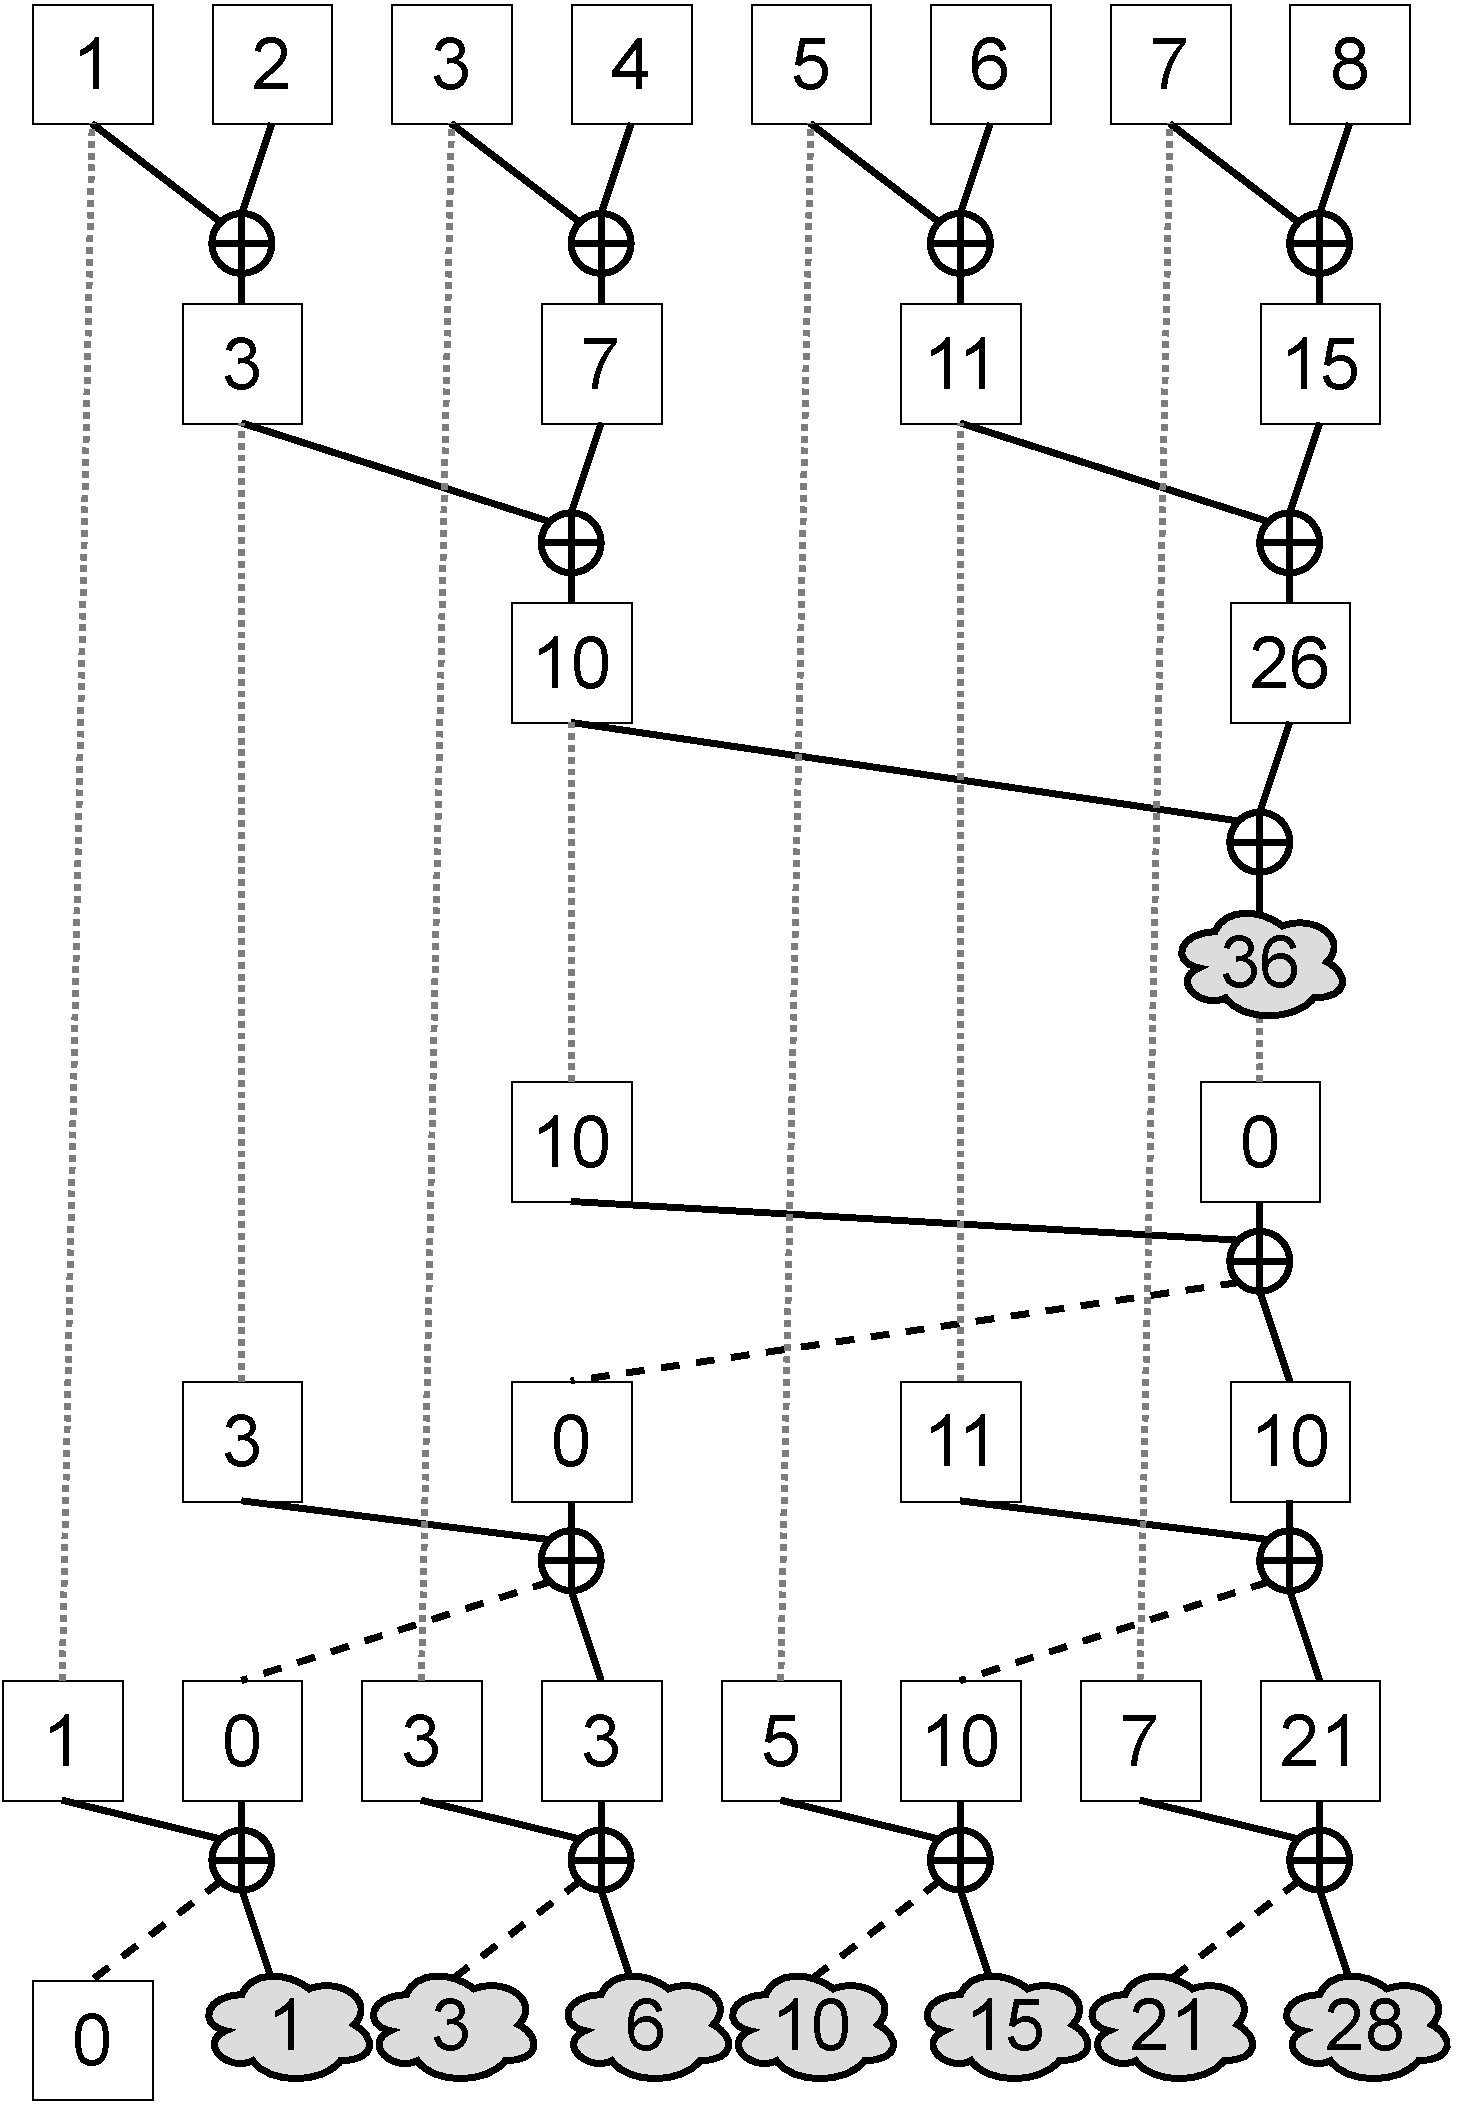
\includegraphics[height=0.3\textheight]{figures/scan_integer.pdf}
    \caption{\textbf{Left:} parallel scan with a generic monoid. \textbf{Right:} illustration on the spetial case of natural integers.}
    \label{fig:parallel_scan_general}
\end{figure}

The procedure described above yields $(\sum_{j=0}^{i-1}a_j)_{i\in I}$, with the cumulative sum being $a^{\log_2(T)}_{0}$ the intermediate result of the upward sweep. We analyse the work complexity $W$ and the time complexity $T_\infty$ of $\mathrm{Scan}$ in terms of floating point operations, where $W$ counts the total number of operations needed and $T_\infty$ counts the time complexity under unlimited parallelism.

\begin{proposition}[Parallel Scan Complexity for Integers]
\label{prop:scan_integer_complexity}
    Let $(M, \oplus, e) \coloneqq (\N, +, 0)$ be the monoid of natural integers equipped with addition. Let $(a_i)_{i\in I}\in \N^I$ be a sequence of integers.

\begin{align}
    W(\mathrm{Scan})&= 2(T-1)\\
    T_\infty(\mathrm{Scan})&= 2\log_2 T
\end{align}
\end{proposition}

\begin{proof}
At level $l$ of the upward scan, $U_l = T/(2^{l+1})$ $\oplus$ operations are performed, each of them having a complexity of $1$. There are $\log_2 T$ levels in total. The same goes on for the downward scan, with $D_l = T/(2^{\log_2(T) - l})=2^{l}$ operations at level $l$. Therefore, the work complexity of level $l$ is $U_l$ (resp. $D_l$) while its time complexity is $1$ with unlimited parallelism. It follows that

\begin{align}
\label{eq:W_integer}
W &= 2\sum_{l=0}^{\log_2(T)-1}2^l=2(T-1)\\
\label{eq:T_integer}
T_\infty&= 2\sum_{l=0}^{\log_2(T)-1}1=2\log_2T
\end{align}
\end{proof}

The key point of this analysis is that the $\oplus$ operation has constant time complexity.

\subsection{SSM Complexity}
\label{app:SSM_complexity}

The case of SSMs is a little more complicated than that of real numbers. In SSMs, the recurrence is defined by \Cref{eq:ssm:recurrence}. We take $B = I$ and $d = N$ for simplicity. Thus, the goal is to compute in parallel the hidden states $(h_i = \sum_{j=0}^i\overline{A}^{i-j}x_j)_i\in I$, where $x_i$ are vectors of dimension $d$ and $\overline{A}$ is a square matrix. This is almost but not quite what we need for the parallel scan. We define the following monoid:
\begin{align}
\label{eq:M_SSM}
    &M^{\mathrm{SSM}}\coloneqq \left\{a = (A, x)\mid A\!\in\!\mathcal{M}_{d}(\R),~x\!\in\!\R^d\right\}\\
\label{eq:+_SSM}
    &(A_a, x_a) \oplus^{\mathrm{SSM}} (A_b,x_b)\coloneqq (A_b \odot A_a, A_b \cdot x_a + x_b)\\
\label{eq:0_SSM}
    &e^{\mathrm{SSM}}\coloneqq(I_d, 0)
\end{align}

With this monoid structure, and the sequence $(a_t)_{t\in I} \coloneqq ((\overline{A}_t, x_t))_{t\in I} \in M^I$, the result of the parallel scan is $((A^t, \sum_{j=0}^tA^{t-j}x_j))_{t\in I}$. The complexity of the scan is less straightforward, but the complexity of each $\oplus^{\mathrm{SSM}}$ operation depends only on $d$. It is a constant of $T$. Therefore, the overall time complexity of the scan is $T_\infty= O(\log T)$ and $W=O(T)$.

\begin{proposition}[SSM Complexity]
    Let $(M, \oplus) \coloneqq (M^{\mathrm{SSM}}, \oplus^{\mathrm{SSM}})$ be the monoid defined by \Cref{eq:M_SSM,eq:+_SSM,eq:0_SSM}. Let $(a_i)_{i\in I}\in (M^{\mathrm{SSM}})^I$.

\begin{align}
    W(\mathrm{Scan})&= 2(T-1)(d^3+d^2+d)\\
    T_\infty(\mathrm{Scan})&= 2\log_2 (T) (d^3+d^2+d)
\end{align}
\end{proposition}

\begin{proof}
The proof of \Cref{prop:scan_integer_complexity} applies with the only difference that now, each $\oplus^{\mathrm{SSM}}$ operation has complexity $d^3$ for the matrix multiplication on the left, $d^2$ for the matrix-vector multiplication and $d$ for the vector addition on the right.
\end{proof}

\subsection{Spatial ConvSSM Complexity}
\label{app:Spatial_ConvSSM_complexity}

Rewriting the SSM (\Cref{eq:ssm:recurrence}) to the ConvSSM formulation of \Cref{eq:conv_ssm_discrete}, we can similarly adapt the monoid structure as :
\begin{align}
    &M^{\mathrm{Conv}_1}\coloneqq \left\{a = (K, x)\mid \exists k_1, k_2,\quad K\!\in\!\R^{k_1\times k_2\times c\times c},~x\!\in\!\R^{h \times w \times c}\right\}\\
    &(K_a, x_a) \oplus^{\mathrm{Conv}_1} (K_b,x_b)\coloneqq (K_b \circledast K_a, K_b \ast x_a + x_b)\\
    &e^{\mathrm{Conv}_1}\coloneqq(I, 0)
\end{align}
\noindent where $\circledast$ is the block convolution between two kernels and $\ast$ is the convolution between a kernel and an image:

\begin{align*}
    & \forall \left\{
\begin{aligned}
    &i\!\in\!\intint{0}{h\!-\!1}\\
    &j\!\in\!\intint{0}{w\!-\!1}\\
    &c_{\mathrm{out}}\!\in\!\intint{1}{c}
\end{aligned}
\right., (K\!\ast\!x)_{i,j,c_{\mathrm{out}}} = \sum_{u=0}^{k_1-1}\sum_{v=0}^{k_2-1}\sum_{c_{\mathrm{in}}=1}^{c} K_{u,v,c_{\mathrm{in}},c_{\mathrm{out}}} x_{(i-u,j-v)\%(h,w),c_{\mathrm{in}}}\\
    & \forall \left\{
\begin{aligned}
    &u\!\in\!\intint{0}{k_1\!+\!l_1\!-\!2}\\
    &v\!\in\!\intint{0}{k_2\!+\!l_2\!-\!2}\\
    &c_{\mathrm{in}},c_{\mathrm{out}}\!\in\!\intint{1}{c}
\end{aligned}
\right., (L \circledast K)_{u,v,c_{\mathrm{in}},c_{\mathrm{out}}} = \sum_{p=0}^{l_1-1}\sum_{q=0}^{l_2-1}\sum_{c_{k}=1}^{c} L_{p,q,c_{k},c_{\mathrm{out}}} K_{u-p,v-q,c_{\mathrm{in}},c_{k}}\text{, $K$ being zero-padded}
\end{align*}
\noindent with $L\!\in\!\R^{l_1\times l_2\times c \times c}$, $K\!\in\!\R^{k_1\times k_2\times c \times c}$ and $x\!\in\!\R^{h \times w \times c}$.

With this structure, the key aspect is that the spatial size of the kernel resulting from $\circledast$ is the sum of the sizes of the input kernels. Therefore, the parallel scan algorithm operates on larger and larger kernel sizes, with sizes growing exponentially with the depth in the tree structure. The complexity of the $\oplus^{\mathrm{Conv}_1}$ operator is thus no more constant as it depends on the depth. The bottleneck is at the very last layer of the upward scan, where kernel size is $O(Tk)$, with $k$ the size of the original kernels $\overline{K}_t$, resulting in a single $\ast$ operation whose complexity is in $O(T^2)$. This bottleneck is illustrated in \Cref{fig:parallel_scan_conv_spatial}.

\begin{proposition}[Spatial ConvSSM Complexity]
    Let $(M, \oplus) \coloneqq (M^{\mathrm{Conv}_1}, \oplus^{\mathrm{Conv}_1})$ be the monoid defined by \Cref{eq:M_SSM,eq:+_SSM,eq:0_SSM}. Let $(a_i)_{i\in I}\in (M^{\mathrm{Conv}_1})^I$.

\begin{align}
    W&= O(T^2)\\
    T_\infty&= O(W)
\end{align}
\end{proposition}

\begin{proof}
The proof of \Cref{prop:scan_integer_complexity} applies with the major difference that in the upward scan, at level $l$, each $\oplus^{\mathrm{Conv}_1}$ operation has complexity $(k+(2^l-1)(k-1))^2 \times c^3 = O((2^l)^2\times k^2 \times c^3)$ for the kernel-kernel convolution on the left, $O(h w \times (2^l)^2 k^2 \times c^2)$ for the kernel-image convolution and $h w c$ for the image addition on the right. The same goes on for the downward scan.

Thus, \Cref{eq:W_integer,eq:T_integer} become :

\begin{align}
\label{eq:W_conv}
W &= O(2 \sum_{l=0}^{\log_2(T)-1} 2^{\log_2(T)-(l+1)} \times \left[ (2^l)^2 k^2 \times c^3 + h w \times (2^l)^2 k^2 \times c^2\right])\\
&= O(T^2 \times k^2 \times c^3) + O(T^2 \times h w \times k^2 \times c^2)\\
\label{eq:T_conv}
T_\infty&= O(2\sum_{l=0}^{\log_2(T)-1} \left[ (2^l)^2 k^2 \times c^3 + h w \times (2^l)^2 k^2 \times c^2\right])\\
&= O(W)
\end{align}
\end{proof}

\begin{figure}[ht]
    \centering
    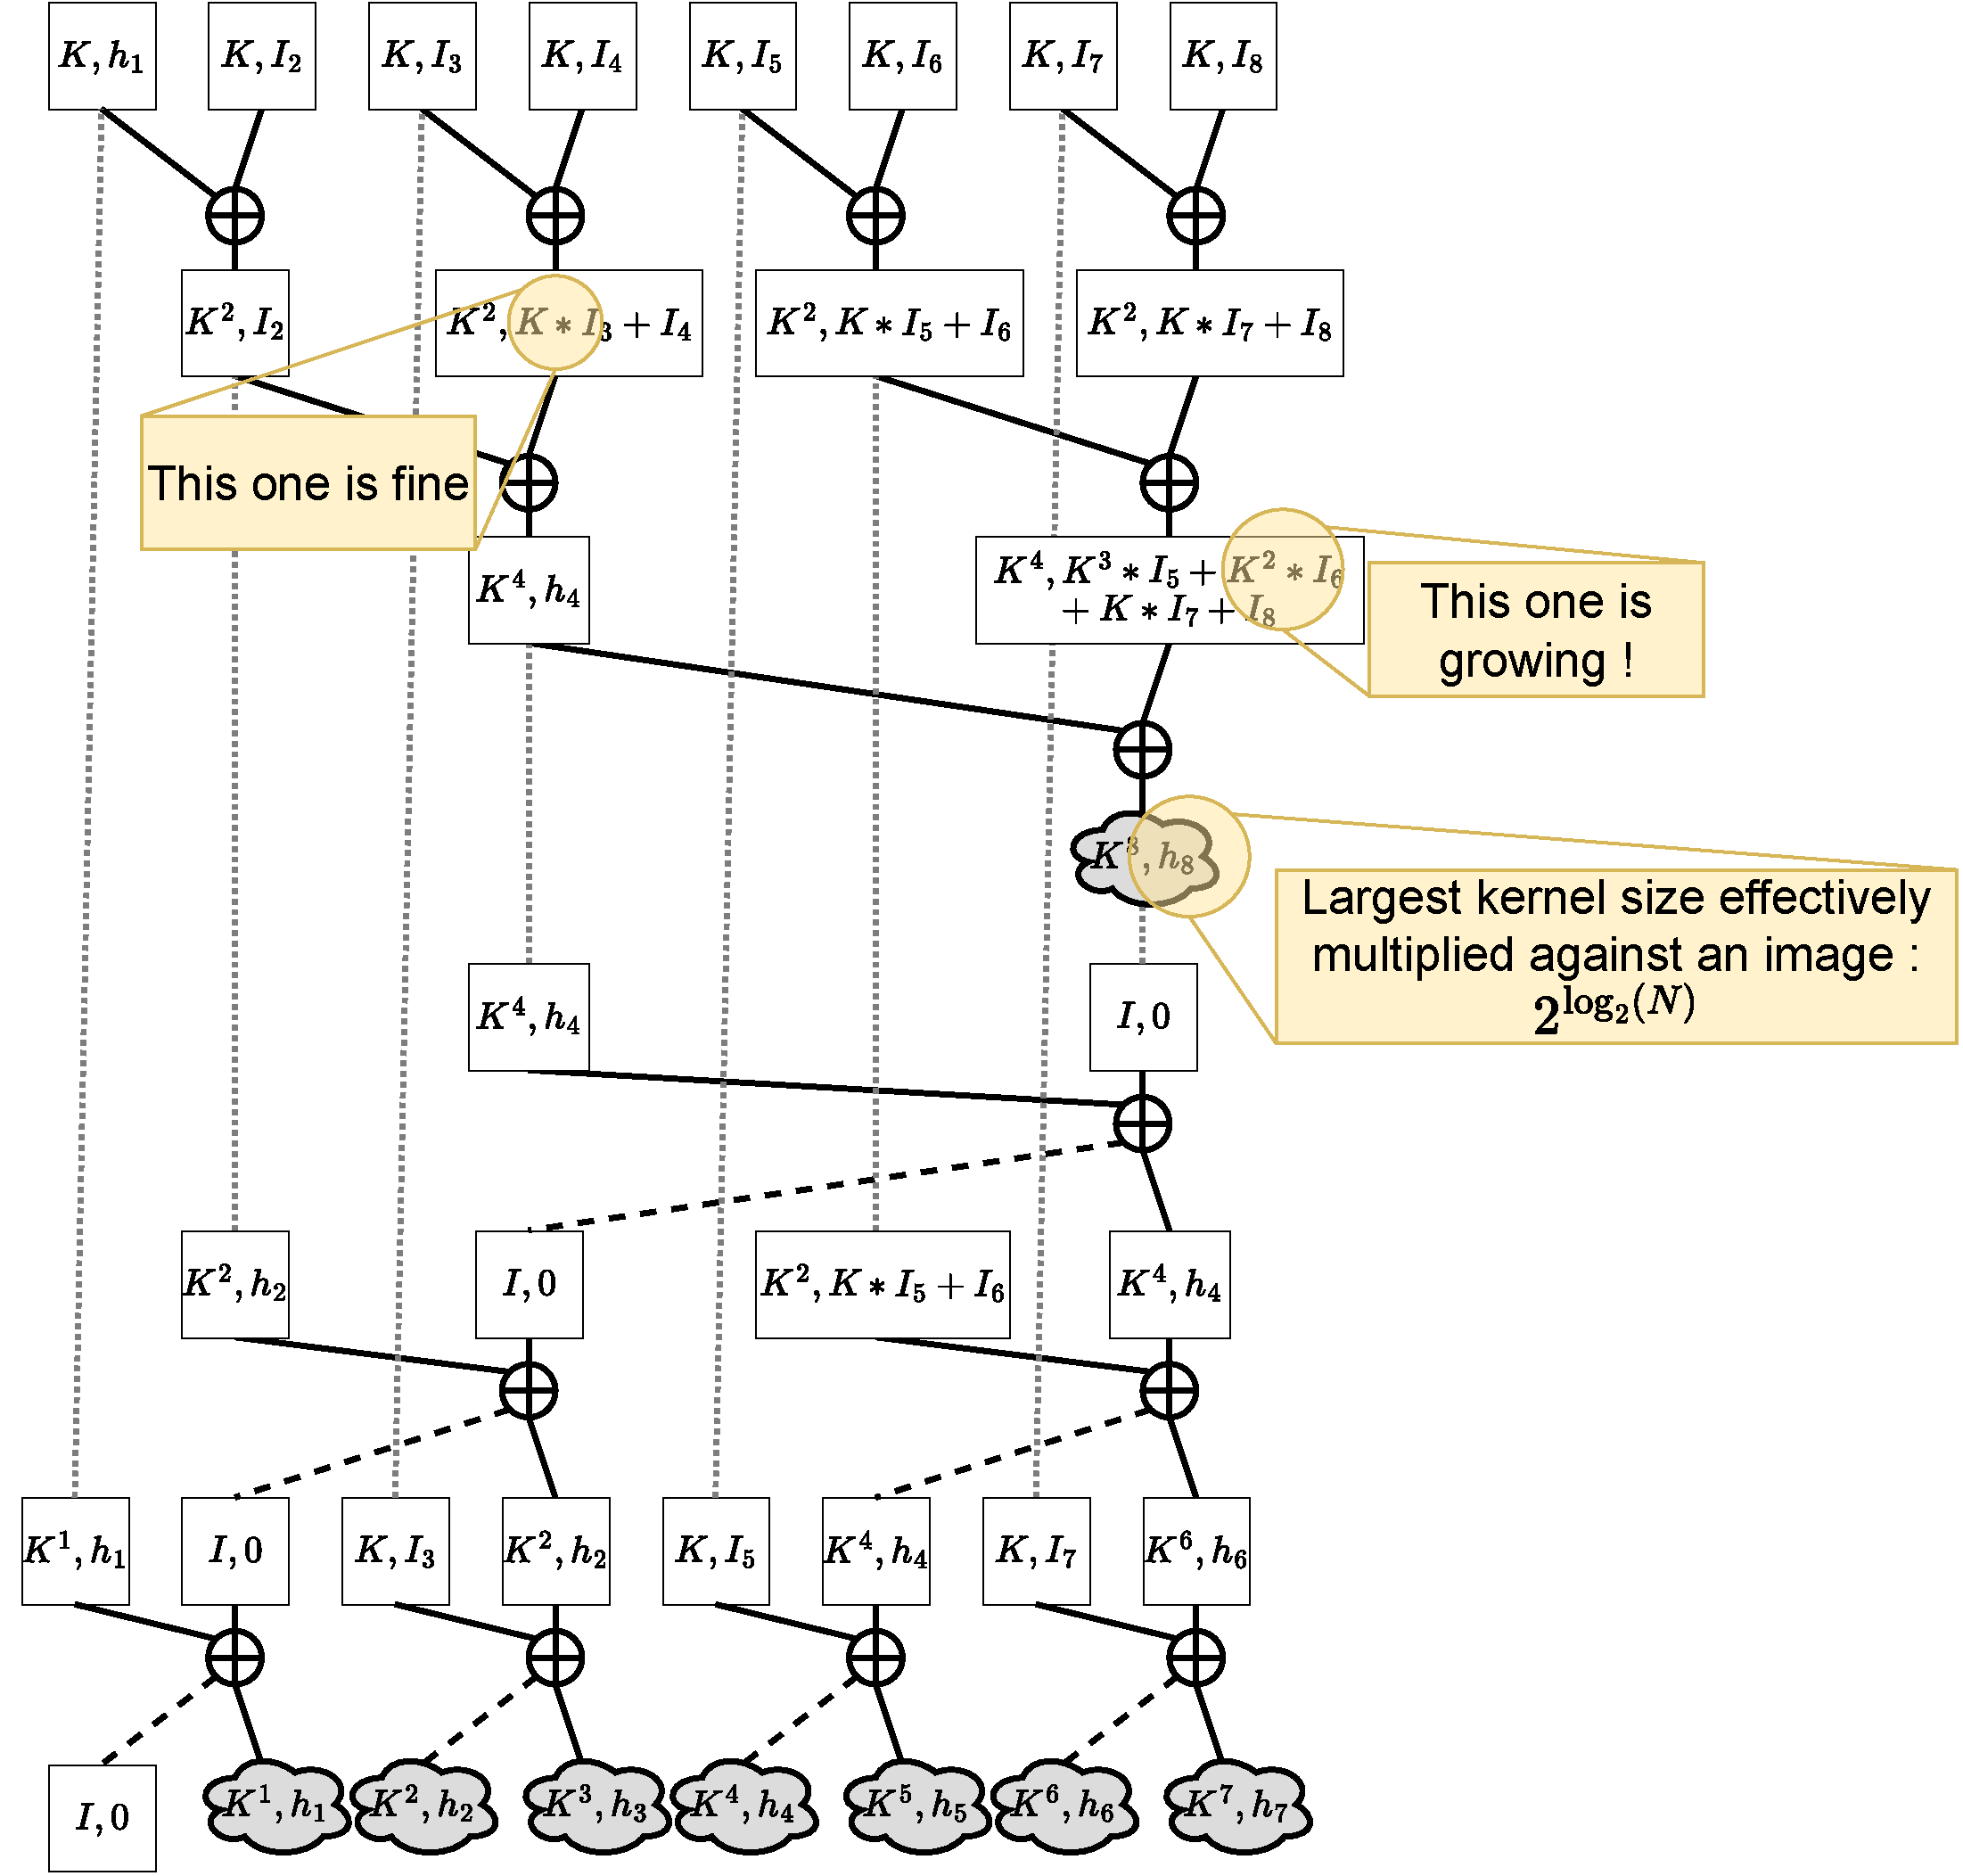
\includegraphics[height=0.3\textheight]{figures/scan_conv.pdf}
    \caption{Parallel scan applied to the monoid structure defined for spatial convolution SSM. Highlighted is the core of the issue : growing kernels lead to a bottleneck where a single operation has $O(T^2)$ complexity.}
    \label{fig:parallel_scan_conv_spatial}
\end{figure}

Moreover, as mentioned in the main text, the discretization step of the SSM leads to kernels with full spatial support, meaning that the initialization of the scan is $(a_t)_{t\in I} = ((\overline{K}_t, x_t))_{t\in I}$ with $\overline{K}_t$ of size $h \!\times\! w$. Thus, even the first step of the scan is intractable.

\subsection{Spectral ConvSSM Complexity}
\label{app:Spectral_ConvSSM_complexity}

To dispell the curse of growing kernels we move to the spectral domain and the ConvSSM formulation of \Cref{eq:convssm}. In this domain, our monoid becomes:
\begin{align}
\label{eq:M_SSM_spectral}
    &M^{\mathrm{Conv}_2}\coloneqq \left\{ a = (\Lambda_c, x)\,\middle|\,\exists (K, x')\in M^{\mathrm{Conv}_1},\Bigl\{
\begin{aligned}
    &\Lambda_c = P^{-1} \mathrm{Circ}(K_{\mathrm{padded}}) P \in \C^{hwc \times hwc}\\
    &x = P^{-1} x' \in \C^{h w c}
\end{aligned}
\Bigr.\right\}\\
\label{eq:+_SSM_spectral}
    &(\Lambda^a_c, x_a) \oplus^{\mathrm{Conv}_2} (\Lambda^b_c, x_b)\coloneqq (\Lambda^b_c \odot \Lambda^a_c, \Lambda^b_c \cdot x_a + x_b)\\
\label{eq:0_SSM_spectral}
    &e\coloneqq(I, 0)
\end{align}
\noindent with $\odot$ the element-wise matrix multiplication and $\cdot$ the element-wise matrix-vector multiplication. With this operator, the kernel grows no more, the cost is again a constant of time and depth, depending only on $h$, $w$ and $c$. We are thus back to a time complexity for the parallel scan of $O(\log T)$.

\begin{proposition}[Spectral ConvSSM Complexity]
    Let $(M, +) \coloneqq (M^{\mathrm{Conv}_2}, \oplus^{\mathrm{Conv}_2})$ be the monoid defined by \Cref{eq:M_SSM_spectral,eq:+_SSM_spectral,eq:0_SSM_spectral}. Let $(a_i)_{i\in I}\in (M^{\mathrm{Conv}_2})^I$.

\begin{align}
    W&= O(T)\\
    T_\infty&= O(\log_2T)
\end{align}
\end{proposition}

\begin{proof}
The proof of \Cref{prop:scan_integer_complexity} applies with the only difference that now, each $\oplus^{\mathrm{Conv}_2}$ operation has complexity $h w c^3$ for the kernel-kernel multiplication on the left, $h w c^2$ for the kernel-image multiplication and $h w c$ for the image addition on the right. This gives :

\begin{align}
\label{eq:W_spectral}
    W&= O(T \times h w c^3)\\
\label{eq:T_spectral}
    T_\infty&= O(\log_2T \times h w c^3)
\end{align}
\end{proof}

\subsection{Taking down the constant factors}
\label{app:constant_factors}

Now that we have solved the main issue of complexity explosion with time, we tackle the problem of the constant factor. As mentioned in \Cref{prop:SSM_complexity}, as is, the work complexity is $O(T)$ with a constant that is $O(d^3)$ due to matrix multiplications.
%
The diagonal SSM (\Cref{eq:ssm:diagonal}) reduces this constant from $O(d^3)$ to $O(d)$. The complexity gain comes from the change of basis being absorbed outside of the recurrence such that the recurrence can operate on diagonalized matrices.

In the case of the Spectral SSM (\Cref{eq:ssm:spectral}), the $O(c^3)$ is even more prohibitive as it is repeated over each pixel position, with the total constant being $O(hwc^3)$ in the spectral domain (\Cref{eq:W_spectral,eq:T_spectral}). Hence the diagonal spectral SSM (\Cref{eq:ssm:diagonal_spectral}), which reduces the constant to $O(hwc)$. Our ConvSSM formulation (\Cref{eq:convssm}) exploits this diagonal spectral SSM and couples it with convolutional input and output transforms in order to make the whole model tractable.

\end{document}
